% Created 2021-02-24 Wed 19:22
% Intended LaTeX compiler: pdflatex
\documentclass[11pt]{article}
\usepackage[utf8]{inputenc}
\usepackage[T1]{fontenc}
\usepackage{graphicx}
\usepackage{grffile}
\usepackage{longtable}
\usepackage{wrapfig}
\usepackage{rotating}
\usepackage[normalem]{ulem}
\usepackage{amsmath}
\usepackage{textcomp}
\usepackage{amssymb}
\usepackage{capt-of}
\usepackage{hyperref}
\usepackage{minted}
\usepackage[margin=1in]{geometry}
\usepackage{subcaption}
\author{A. Bochkarev}
\date{}
\title{Facility Location with BDDs: Status update.}
\hypersetup{
 pdfauthor={A. Bochkarev},
 pdftitle={Facility Location with BDDs: Status update.},
 pdfkeywords={},
 pdfsubject={},
 pdfcreator={Emacs 28.0.50 (Org mode 9.4.3)}, 
 pdflang={English}}
\begin{document}

\maketitle

\section{Status}
\label{sec:org1999b84}
\begin{itemize}
\item I have implemented some of the key machinery, so now I can play with it:
weighted BDD transformations, building a simple MIP, creating BDDs
(availability, covering, and their intersection), building CPP MIP and a
network flow based on the intersection BDD.
\item I ran several really simple examples, and stumbled upon a problem: I think
my intersection BDD (unsurprisingly) blows up. It is a little more dramatic
than I expected: I'd need to find a way to make instances large enough
to be difficult for MIP, but still tractable by BDDs (see the last section
here).
\end{itemize}

\section{A toy example (updated, again)}
\label{sec:org0063178}
This is a simple example updated in the spirit of our recent discussions.
\subsection{Problem description}
\label{sec:org94cda4c}
Let us consider a simple problem with two facilities and three customers, as
depicted in Figure \ref{fig:problem}.

\begin{figure}[h!]
\center
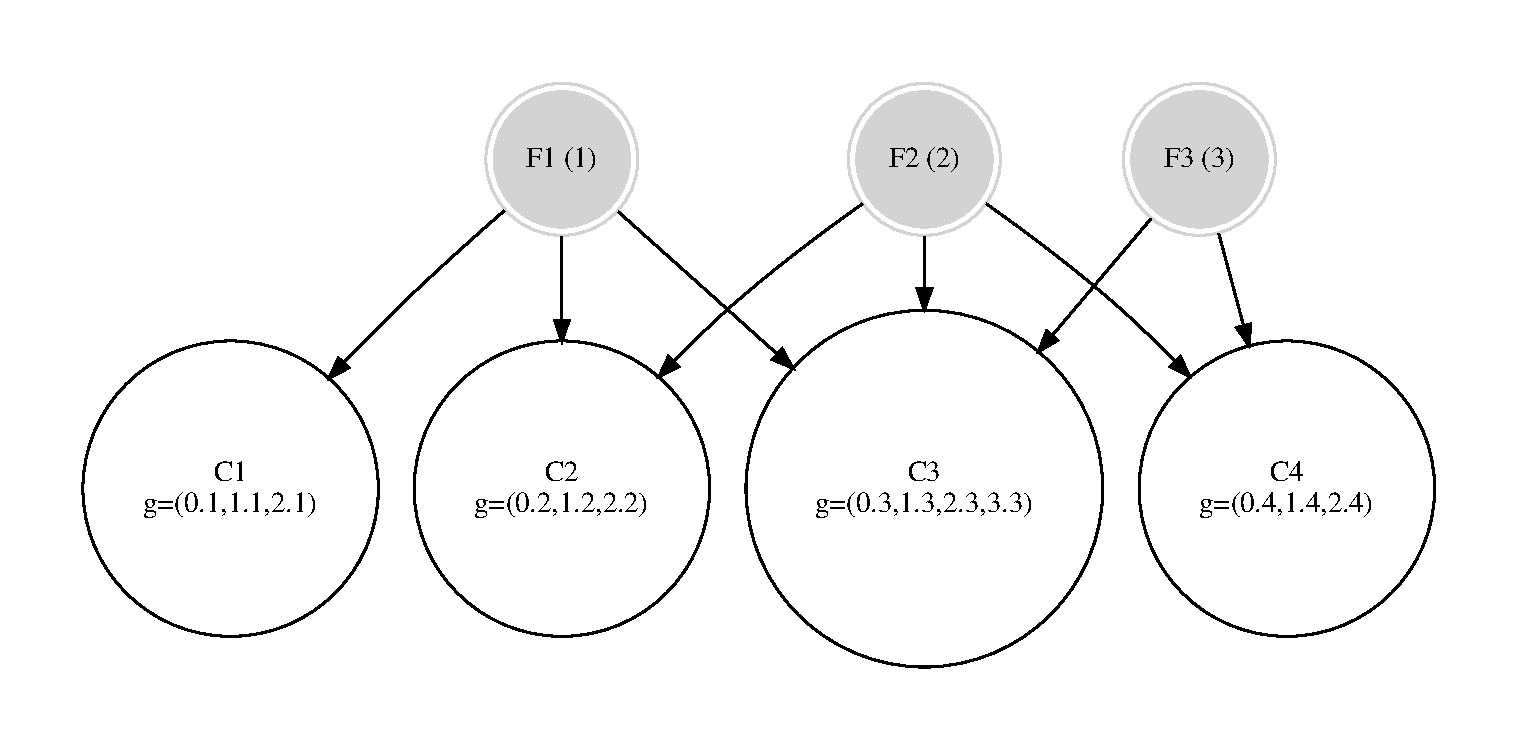
\includegraphics[width=0.8\textwidth]{./problem_dia.gv.pdf}
\caption{Problem description: facilty location with overlaps. \\
\textbf{Facilities:} numbers in parentheses indicate locating (``turn-on'') costs.\\
\textbf{Consumers:} overlap penalies are shown, $g=(0,1,2)$ would mean that for this consumer zero
overlapping coverings imposed no additional cost, covering with one facility brought additional cost $1$,
with two facilities (i.e., actual overlap) brought cost $2$.}
\label{fig:problem}
\end{figure}

I am representing this (or any other) problem in the following three ways.
\subsection{Simple MIP}
\label{sec:org71b1d70}
I generate a "naive" MIP right away:
\begin{flalign*}
    \textrm{Minimize:} & 50.0 + x_{1} + 2.0 x_{2} + 3.0 x_{3} -11.0 v^1_1 -12.0 v^1_2 + 2.2 v^2_2 -13.0 v^1_3 + 2.3 v^2_3 + 0.8 v^3_3 -14.0 v^1_4 + 2.4 v^2_4\\
    \textrm{Subject To:} &\\
& -1.0 x_{1} + z_{1\rightarrow 1} = 0.0\\
& -1.0 x_{1} + z_{1\rightarrow 2} = 0.0\\
& -1.0 x_{1} + z_{1\rightarrow 3} = 0.0\\
& -1.0 x_{2} + z_{2\rightarrow 2} = 0.0\\
& -1.0 x_{2} + z_{2\rightarrow 3} = 0.0\\
& -1.0 x_{2} + z_{2\rightarrow 4} = 0.0\\
& -1.0 x_{3} + z_{3\rightarrow 3} = 0.0\\
& -1.0 x_{3} + z_{3\rightarrow 4} = 0.0\\
& -1.0 z_{1\rightarrow 1} + b_{1} = 0.0\\
& -1.0 z_{1\rightarrow 2} -1.0 z_{2\rightarrow 2} + b_{2} = 0.0\\
& -1.0 z_{1\rightarrow 3} -1.0 z_{2\rightarrow 3} -1.0 z_{3\rightarrow 3} + b_{3} = 0.0\\
& -1.0 z_{2\rightarrow 4} -1.0 z_{3\rightarrow 4} + b_{4} = 0.0\\
& b_{1} -1.0 v^1_1 = 0.0\\
& -1.0 v^1_2 + v^2_2 \leq 0.0\\
& b_{2} -1.0 v^1_2 -1.0 v^2_2 = 0.0\\
& -1.0 v^1_3 + v^2_3 \leq 0.0\\
& -1.0 v^2_3 + v^3_3 \leq 0.0\\
& b_{3} -1.0 v^1_3 -1.0 v^2_3 -1.0 v^3_3 = 0.0\\
& -1.0 v^1_4 + v^2_4 \leq 0.0\\
& b_{4} -1.0 v^1_4 -1.0 v^2_4 = 0.0,
\end{flalign*}
where \(x\) are "locate" decisions, \(z\) are covering decisions (which are kind of
dependent on each other, like we discussed), \(b\) are numbers of overlaps, and
\(v\) are used to encode an arbitrary overlap penalty function \(v^k_j\) corresponds
to customer \(j\) being "overlapped" \(k\) times.

Binary variables are: \(x_{1}, z_{1\rightarrow 1}, z_{1\rightarrow 2},
z_{1\rightarrow 3}, x_{2}, z_{2\rightarrow 2}, z_{2\rightarrow 3},
z_{2\rightarrow 4}, x_{3}, z_{3\rightarrow 3}, z_{3\rightarrow 4}, v^1_1, v^1_2,
v^2_2, v^1_3, v^2_3, v^3_3, v^1_4, v^2_4\) (and I kind of hope that Gurobi's
\texttt{presolve} takes care of the redundant variables.)

\subsection{CPP MIP}
\label{sec:org0964bed}
Now, I am generating two decision diagrams, as before:

\begin{center}
\begin{tabular}{llll}
\textbf{Diagram} & \textbf{Constraints incorporated} & \textbf{Costs incorporated} & \textbf{Figure}\\
\hline
\hline
Covering & (Costs for) covering each & \(g_j(n_j)\) (overlap) & \ref{fig:cover}\\
 & consumer -- nothing hard. &  & \\
\hline
Availability & "Turn on" and "covering" & \(f_i\) (location) & \ref{fig:avail}\\
 & variables are consistent &  & \\
\hline
\end{tabular}
\end{center}

\begin{figure}[t!]
  \begin{subfigure}[t]{0.45\textwidth}
    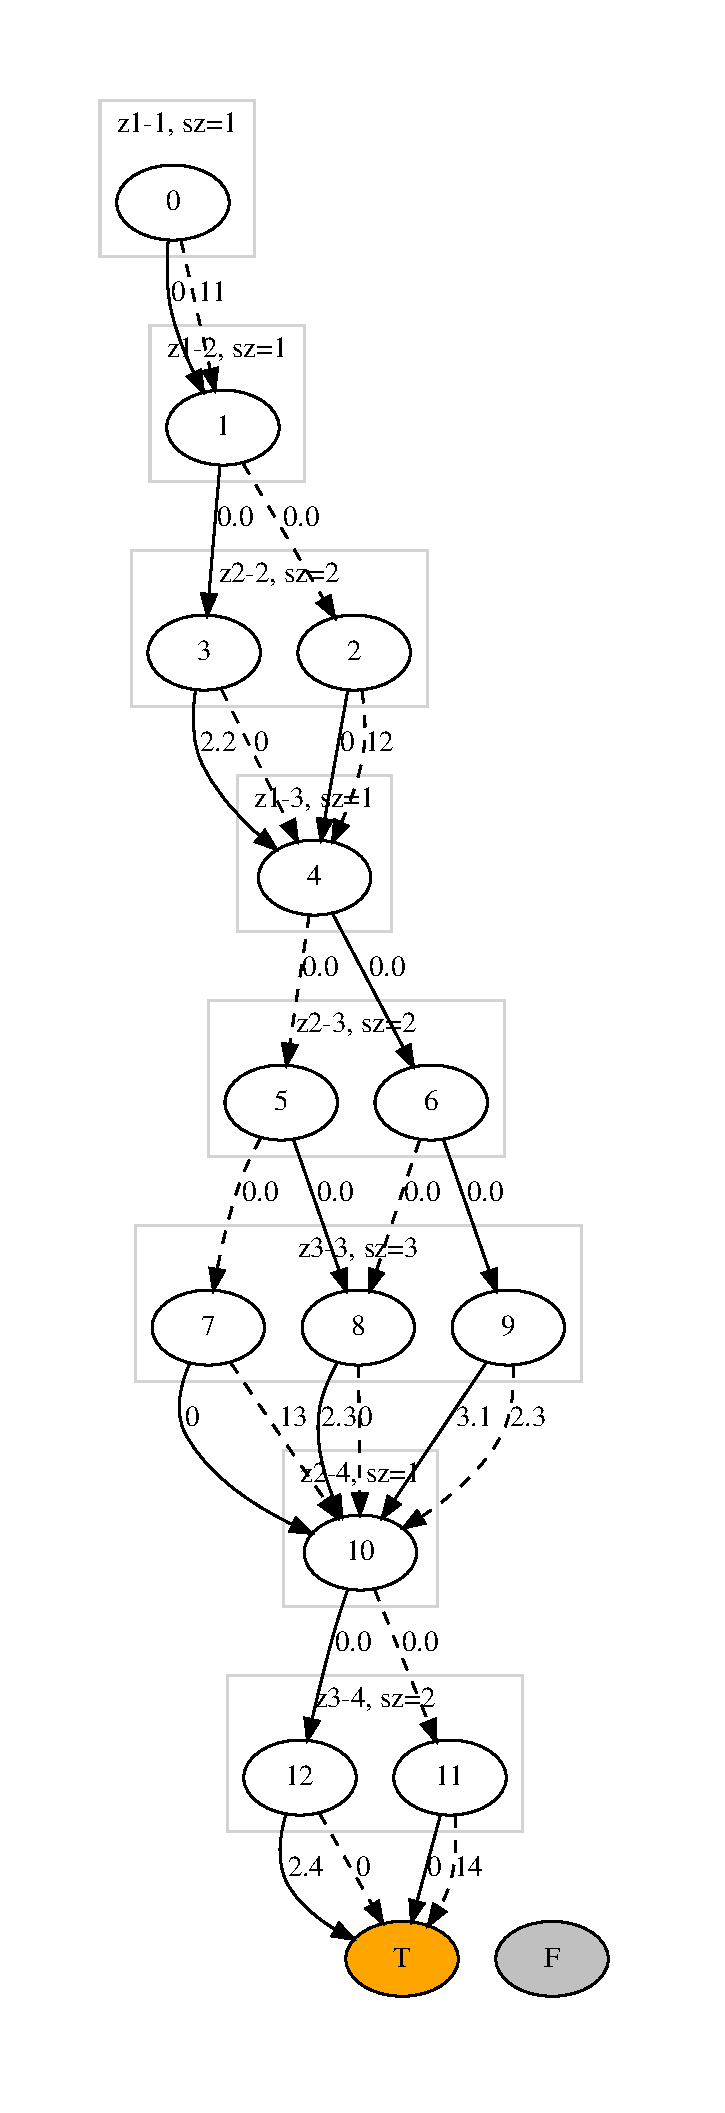
\includegraphics[height=\textheight]{./covering.dot.pdf}
    \caption{Covering BDD}\label{fig:cover}
  \end{subfigure}%
  \hfill
  \begin{subfigure}[t]{0.45\textwidth}
    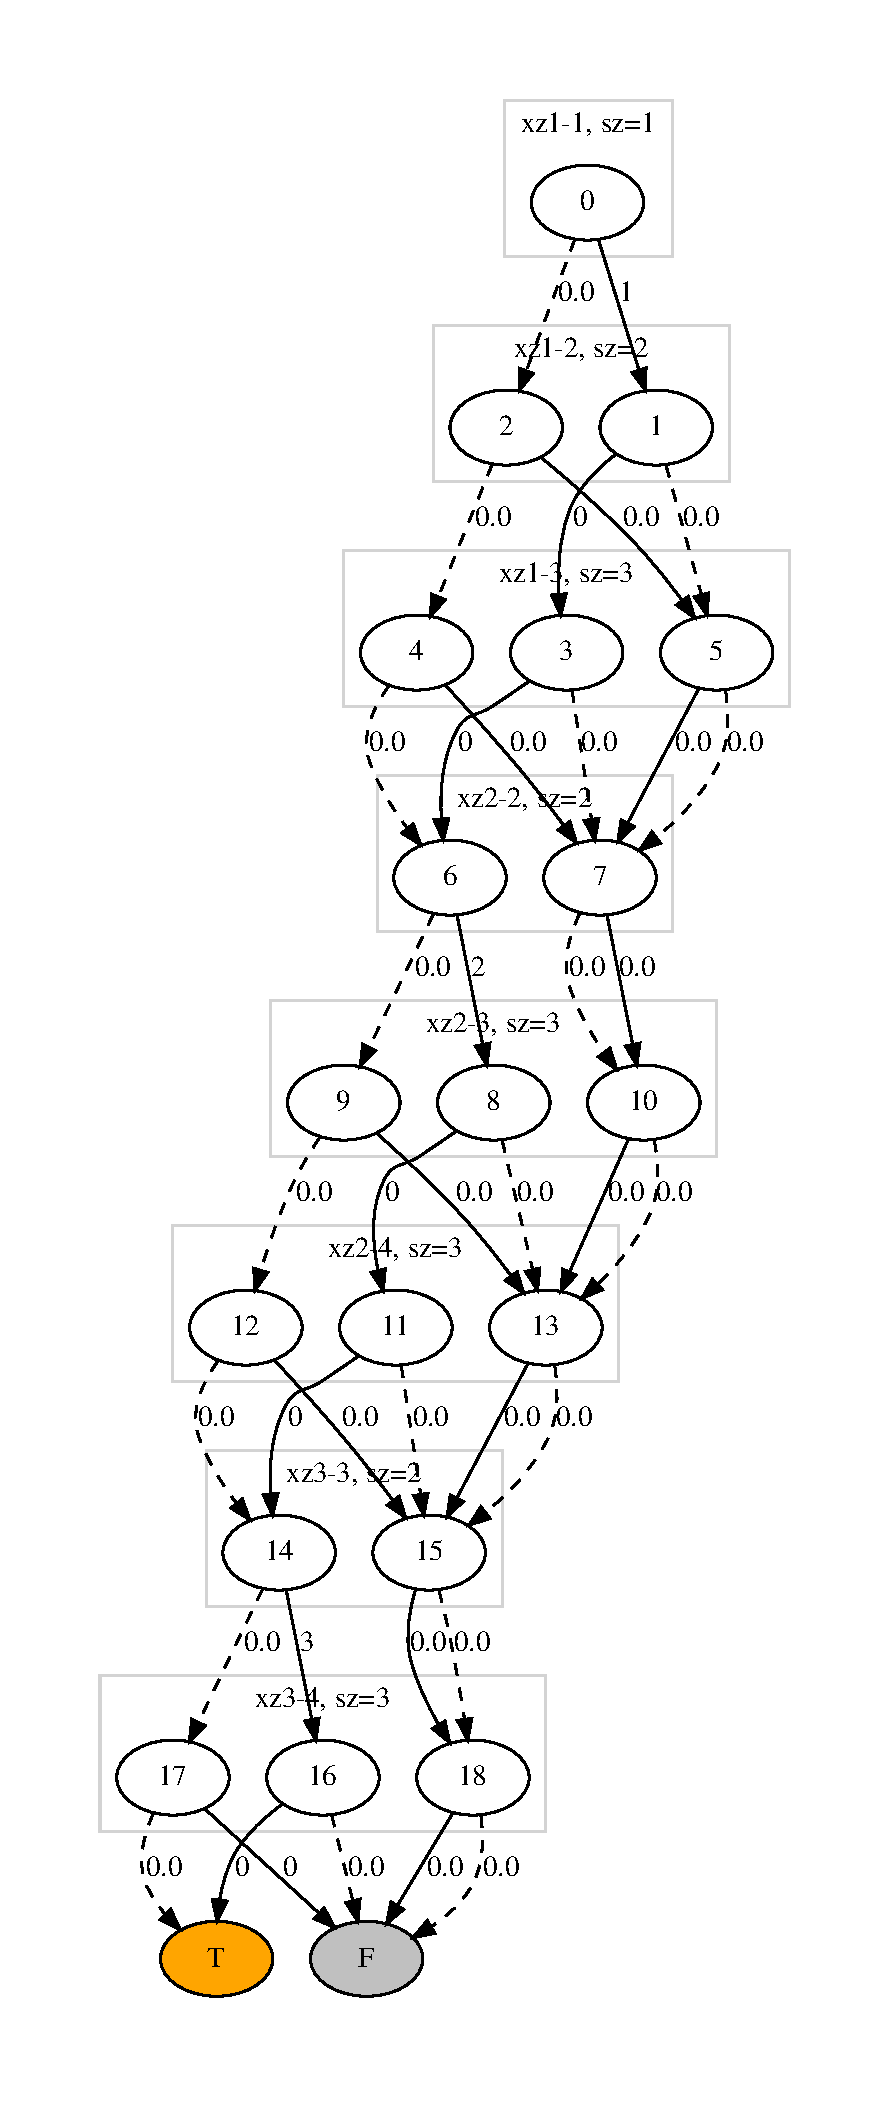
\includegraphics[height=\textheight]{./availability.dot.pdf}
    \caption{Availability BDD}\label{fig:avail}
  \end{subfigure}
  \caption{BDDs generated to encode the instance from Figure \ref{fig:problem}.}
\end{figure}

Which allows me to formulate the following MIP:
The objective is:
\begin{flalign*}
\textrm{Minimize:}\quad\quad & v^A_{0\rightarrow 1,h} + 2.0 v^A_{6 \rightarrow 8, h} + 3.0 v^A_{14 \rightarrow 16, h} + 11.0 v^C_{0 \rightarrow 1, l} + 2.2 v^C_{3 \rightarrow 4, h} + 12.0 v^C_{2 \rightarrow 4, l} + 3.1 v^C_{9 \rightarrow 10, h} + \\
& 2.3 v^C_{9 \rightarrow 10, l} + 2.3 v^C_{8 \rightarrow 10, h} + 13.0 v^C_{7 \rightarrow 10, l} + 2.4 v^C_{12 \rightarrow T, h} + 14.0 v^C_{11 \rightarrow T, l}.
\end{flalign*}

Here, for example, variable \(v^A_{0\rightarrow 1,h}\) corresponds to the flow
from node \textcircled{0} to node \textcircled{1} of diagram \(A\) (availability),
along the "hi" ("yes") arc.\\

\textbf{Legend.}
\begin{itemize}
\item From each diagram, two types of constraints are generated:
\begin{itemize}
\item \emph{cont-at-\textcircled{.}} are flow continuity constraints at a given node.
\item \emph{bin-link-<k>} are binary linking constraints (needed to link two BDDs -- i.e.,
tangle network flow problems), one per layer, indexed with \(k\).
\end{itemize}
\item \(A\) denotes "Availability" diagram, \(C\) denotes "Covering"
diagram.
\end{itemize}

All node numbers correspond to the diagrams and have nothing to do with
customer and facility indices.

\begin{itemize}
\item Arc flow variables, continuous, \(v\) (sorry, these \(v\) have nothing to do with \(v_j^k\) from the previous section).
\item Linking variables (binary): \(\lambda_{z1-1}, \lambda_{z1-2}, \lambda_{z1-3}, \lambda_{z2-2}, \lambda_{z2-3}, \lambda_{z2-4}, \lambda_{z3-3}, \lambda_{z3-4}\).
\end{itemize}

\newpage Constraints from \textbf{covering BDD}:\\

\begin{tabular}{l l}
\textbf{Type} & \textbf{Constraint}\\\hline\\
   cont-at-0 & $-1.0 v^C_{0 \rightarrow 1, h} -1.0 v^C_{0 \rightarrow 1, l} = -1.0$\\
   bin-link-1 & $\lambda_{z1-1} -1.0 v^C_{0 \rightarrow 1, h} = 0.0$\\
   cont-at-1 & $v^C_{0 \rightarrow 1, h} + v^C_{0 \rightarrow 1, l} -1.0 v^C_{1 \rightarrow 3, h} -1.0 v^C_{1 \rightarrow 2, l} = 0.0$\\
   bin-link-2 & $\lambda_{z1-2} -1.0 v^C_{1 \rightarrow 3, h} = 0.0$\\
   cont-at-3 & $v^C_{1 \rightarrow 3, h} -1.0 v^C_{3 \rightarrow 4, h} -1.0 v^C_{3 \rightarrow 4, l} = 0.0$\\
   cont-at-2 & $v^C_{1 \rightarrow 2, l} -1.0 v^C_{2 \rightarrow 4, h} -1.0 v^C_{2 \rightarrow 4, l} = 0.0$\\
   bin-link-3 & $\lambda_{z2-2} -1.0 v^C_{3 \rightarrow 4, h} -1.0 v^C_{2 \rightarrow 4, h} = 0.0$\\
   cont-at-4 & $v^C_{3 \rightarrow 4, h} + v^C_{3 \rightarrow 4, l} + v^C_{2 \rightarrow 4, h} + v^C_{2 \rightarrow 4, l} -1.0 v^C_{4 \rightarrow 6, h} -1.0 v^C_{4 \rightarrow 5, l} = 0.0$\\
   bin-link-4 & $\lambda_{z1-3} -1.0 v^C_{4 \rightarrow 6, h} = 0.0$\\
   cont-at-5 & $v^C_{4 \rightarrow 5, l} -1.0 v^C_{5 \rightarrow 8, h} -1.0 v^C_{5 \rightarrow 7, l} = 0.0$\\
   cont-at-6 & $v^C_{4 \rightarrow 6, h} -1.0 v^C_{6 \rightarrow 9, h} -1.0 v^C_{6 \rightarrow 8, l} = 0.0$\\
   bin-link-5 & $\lambda_{z2-3} -1.0 v^C_{5 \rightarrow 8, h} -1.0 v^C_{6 \rightarrow 9, h} = 0.0$\\
   cont-at-9 & $v^C_{6 \rightarrow 9, h} -1.0 v^C_{9 \rightarrow 10, h} -1.0 v^C_{9 \rightarrow 10, l} = 0.0$\\
   cont-at-8 & $v^C_{5 \rightarrow 8, h} + v^C_{6 \rightarrow 8, l} -1.0 v^C_{8 \rightarrow 10, h} -1.0 v^C_{8 \rightarrow 10, l} = 0.0$\\
   cont-at-7 & $v^C_{5 \rightarrow 7, l} -1.0 v^C_{7 \rightarrow 10, h} -1.0 v^C_{7 \rightarrow 10, l} = 0.0$\\
   bin-link-6 & $\lambda_{z3-3} -1.0 v^C_{9 \rightarrow 10, h} -1.0 v^C_{8 \rightarrow 10, h} -1.0 v^C_{7 \rightarrow 10, h} = 0.0$\\
   cont-at-10 & $v^C_{9 \rightarrow 10, h} + v^C_{9 \rightarrow 10, l} + v^C_{8 \rightarrow 10, h} + v^C_{8 \rightarrow 10, l} + v^C_{7 \rightarrow 10, h} + v^C_{7 \rightarrow 10, l} -1.0 v^C_{10 \rightarrow 12, h} -1.0 v^C_{10 \rightarrow 11, l} = 0.0$\\
   bin-link-7 & $\lambda_{z2-4} -1.0 v^C_{10 \rightarrow 12, h} = 0.0$\\
   cont-at-12 & $v^C_{10 \rightarrow 12, h} -1.0 v^C_{12 \rightarrow T, h} -1.0 v^C_{12 \rightarrow T, l} = 0.0$\\
   cont-at-11 & $v^C_{10 \rightarrow 11, l} -1.0 v^C_{11 \rightarrow T, h} -1.0 v^C_{11 \rightarrow T, l} = 0.0$\\
   bin-link-8 & $\lambda_{z3-4} -1.0 v^C_{12 \rightarrow T, h} -1.0 v^C_{11 \rightarrow T, h} = 0.0$\\
   cont-at-F & $0.0 = 0.0$\\
   cont-at-T & $v^C_{12 \rightarrow T, h} + v^C_{12 \rightarrow T, l} + v^C_{11 \rightarrow T, h} + v^C_{11 \rightarrow T, l} = 1.0$
\end{tabular}

\newpage Constraints from \textbf{availability BBD}\\

\begin{tabular}{l l}
\textbf{Type} & \textbf{Constraint}\\\hline\\
    cont-at-0 & $-1.0 v^A_{0 \rightarrow 1, h} -1.0 v^A_{0 \rightarrow 2, l} = -1.0$\\
    bin-link-1 & $\lambda_{z1-1} -1.0 v^A_{0 \rightarrow 1, h} = 0.0$\\
    cont-at-1 & $v^A_{0 \rightarrow 1, h} -1.0 v^A_{1 \rightarrow 3, h} -1.0 v^A_{1 \rightarrow 5, l} = 0.0$\\
    cont-at-2 & $v^A_{0 \rightarrow 2, l} -1.0 v^A_{2 \rightarrow 5, h} -1.0 v^A_{2 \rightarrow 4, l} = 0.0$\\
    bin-link-2 & $\lambda_{z1-2} -1.0 v^A_{1 \rightarrow 3, h} -1.0 v^A_{2 \rightarrow 5, h} = 0.0$\\
    cont-at-5 & $v^A_{1 \rightarrow 5, l} + v^A_{2 \rightarrow 5, h} -1.0 v^A_{5 \rightarrow 7, h} -1.0 v^A_{5 \rightarrow 7, l} = 0.0$\\
    cont-at-4 & $v^A_{2 \rightarrow 4, l} -1.0 v^A_{4 \rightarrow 7, h} -1.0 v^A_{4 \rightarrow 6, l} = 0.0$\\
    cont-at-3 & $v^A_{1 \rightarrow 3, h} -1.0 v^A_{3 \rightarrow 6, h} -1.0 v^A_{3 \rightarrow 7, l} = 0.0$\\
    bin-link-3 & $\lambda_{z1-3} -1.0 v^A_{5 \rightarrow 7, h} -1.0 v^A_{4 \rightarrow 7, h} -1.0 v^A_{3 \rightarrow 6, h} = 0.0$\\
    cont-at-6 & $v^A_{4 \rightarrow 6, l} + v^A_{3 \rightarrow 6, h} -1.0 v^A_{6 \rightarrow 8, h} -1.0 v^A_{6 \rightarrow 9, l} = 0.0$\\
    cont-at-7 & $v^A_{5 \rightarrow 7, h} + v^A_{5 \rightarrow 7, l} + v^A_{4 \rightarrow 7, h} + v^A_{3 \rightarrow 7, l} -1.0 v^A_{7 \rightarrow 10, h} -1.0 v^A_{7 \rightarrow 10, l} = 0.0$\\
    bin-link-4 & $\lambda_{z2-2} -1.0 v^A_{6 \rightarrow 8, h} -1.0 v^A_{7 \rightarrow 10, h} = 0.0$\\
    cont-at-8 & $v^A_{6 \rightarrow 8, h} -1.0 v^A_{8 \rightarrow 11, h} -1.0 v^A_{8 \rightarrow 13, l} = 0.0$\\
    cont-at-10 & $v^A_{7 \rightarrow 10, h} + v^A_{7 \rightarrow 10, l} -1.0 v^A_{10 \rightarrow 13, h} -1.0 v^A_{10 \rightarrow 13, l} = 0.0$\\
    cont-at-9 & $v^A_{6 \rightarrow 9, l} -1.0 v^A_{9 \rightarrow 13, h} -1.0 v^A_{9 \rightarrow 12, l} = 0.0$\\
    bin-link-5 & $\lambda_{z2-3} -1.0 v^A_{8 \rightarrow 11, h} -1.0 v^A_{10 \rightarrow 13, h} -1.0 v^A_{9 \rightarrow 13, h} = 0.0$\\
    cont-at-11 & $v^A_{8 \rightarrow 11, h} -1.0 v^A_{11 \rightarrow 14, h} -1.0 v^A_{11 \rightarrow 15, l} = 0.0$\\
    cont-at-13 & $v^A_{8 \rightarrow 13, l} + v^A_{10 \rightarrow 13, h} + v^A_{10 \rightarrow 13, l} + v^A_{9 \rightarrow 13, h} -1.0 v^A_{13 \rightarrow 15, h} -1.0 v^A_{13 \rightarrow 15, l} = 0.0$\\
    cont-at-12 & $v^A_{9 \rightarrow 12, l} -1.0 v^A_{12 \rightarrow 15, h} -1.0 v^A_{12 \rightarrow 14, l} = 0.0$\\
    bin-link-6 & $\lambda_{z2-4} -1.0 v^A_{11 \rightarrow 14, h} -1.0 v^A_{13 \rightarrow 15, h} -1.0 v^A_{12 \rightarrow 15, h} = 0.0$\\
    cont-at-15 & $v^A_{11 \rightarrow 15, l} + v^A_{13 \rightarrow 15, h} + v^A_{13 \rightarrow 15, l} + v^A_{12 \rightarrow 15, h} -1.0 v^A_{15 \rightarrow 18, h} -1.0 v^A_{15 \rightarrow 18, l} = 0.0$\\
    cont-at-14 & $v^A_{11 \rightarrow 14, h} + v^A_{12 \rightarrow 14, l} -1.0 v^A_{14 \rightarrow 16, h} -1.0 v^A_{14 \rightarrow 17, l} = 0.0$\\
    bin-link-7 & $\lambda_{z3-3} -1.0 v^A_{15 \rightarrow 18, h} -1.0 v^A_{14 \rightarrow 16, h} = 0.0$\\
    cont-at-16 & $v^A_{14 \rightarrow 16, h} -1.0 v^A_{16 \rightarrow T, h} -1.0 v^A_{16 \rightarrow F, l} = 0.0$\\
    cont-at-17 & $v^A_{14 \rightarrow 17, l} -1.0 v^A_{17 \rightarrow F, h} -1.0 v^A_{17 \rightarrow T, l} = 0.0$\\
    cont-at-18 & $v^A_{15 \rightarrow 18, h} + v^A_{15 \rightarrow 18, l} -1.0 v^A_{18 \rightarrow F, h} -1.0 v^A_{18 \rightarrow F, l} = 0.0$\\
    bin-link-8 & $\lambda_{z3-4} -1.0 v^A_{16 \rightarrow T, h} -1.0 v^A_{17 \rightarrow F, h} -1.0 v^A_{18 \rightarrow F, h} = 0.0$\\
    cont-at-F & $v^A_{16 \rightarrow F, l} + v^A_{17 \rightarrow F, h} + v^A_{18 \rightarrow F, h} + v^A_{18 \rightarrow F, l} = 0.0$\\
    cont-at-T & $v^A_{16 \rightarrow T, h} + v^A_{17 \rightarrow T, l} = 1.0$
\end{tabular}

\subsection{Intersection BDD}
\label{sec:org0a6546e}
This is a little more tricky. First, I make 'availability' and 'covering' diagrams order-associated:

\begin{minted}[frame=lines,fontsize=\scriptsize,xleftmargin=\parindent,linenos]{python}
import varseq as vs
from BB_search import BBSearch

print(f"Size *before* alignment: {A.size()} + {C.size()} = {A.size() + C.size()} nodes.")
vs_A = vs.VarSeq(A.vars, [len(L) for L in A.layers[:-1]])
vs_C = vs.VarSeq(C.vars, [len(L) for L in C.layers[:-1]])
b = BBSearch(vs_A, vs_C)

status = b.search()
assert status == "optimal" or status == "timeout"

Ap = A.align_to(b.Ap_cand.layer_var, inplace=False)
Cp = C.align_to(b.Ap_cand.layer_var, inplace=False)

Ap.show(dir="reports/2021-02-23_Status_BM/", filename="A_aligned.dot", x_prefix='')
Cp.show(dir="reports/2021-02-23_Status_BM/", filename="C_aligned.dot", x_prefix='')
print(f"Size *after* alignment: {Ap.size()} + {Cp.size()} = {Ap.size() + Cp.size()} nodes.")
print(f"The order revised from \n A: {A.vars}, and\n C: {C.vars}...")
print(f"to: {Ap.vars}")
\end{minted}

\begin{verbatim}
Size *before* alignment: 19 + 13 = 32 nodes.
Size *after* alignment: 22 + 16 = 38 nodes.
The order revised from 
 A: ['z1-1', 'z1-2', 'z1-3', 'z2-2', 'z2-3', 'z2-4', 'z3-3', 'z3-4'], and
 C: ['z1-1', 'z1-2', 'z2-2', 'z1-3', 'z2-3', 'z3-3', 'z2-4', 'z3-4']...
to: ['z1-1', 'z1-2', 'z1-3', 'z2-2', 'z2-3', 'z3-3', 'z2-4', 'z3-4']
\end{verbatim}


(This results in the diagrams depicted in Figures \ref{fig:coverA} and \ref{fig:availA}, respectively.)

\begin{figure}[t!]
  \begin{subfigure}[t]{0.45\textwidth}
    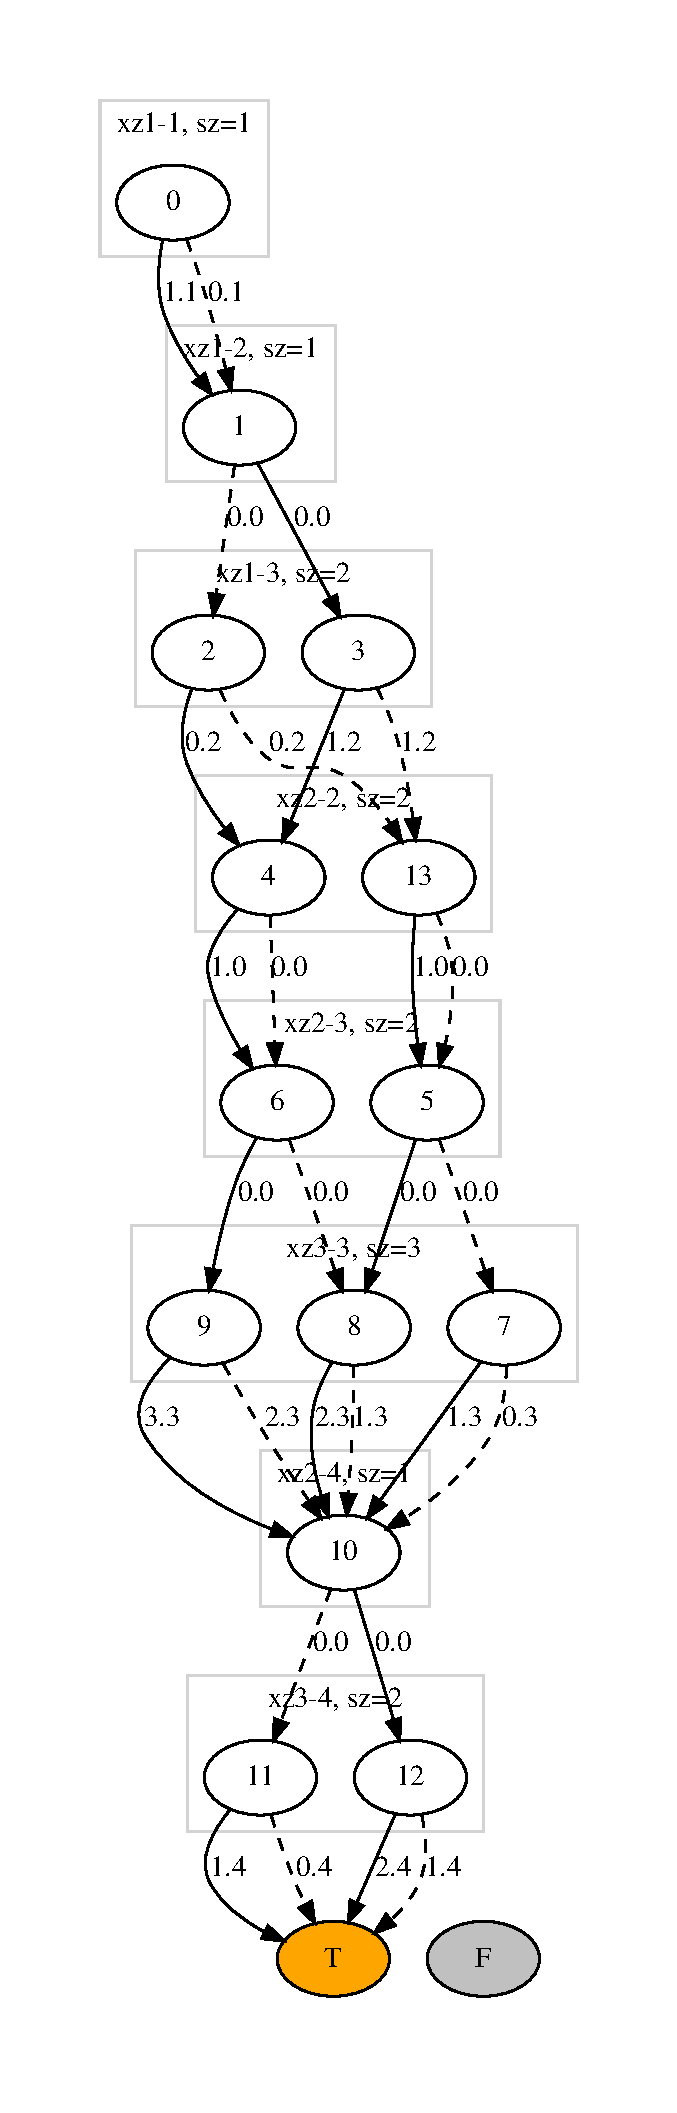
\includegraphics[height=\textheight]{./C_aligned.dot.pdf}
    \caption{Covering BDD}\label{fig:coverA}
  \end{subfigure}%
  \hfill
  \begin{subfigure}[t]{0.45\textwidth}
    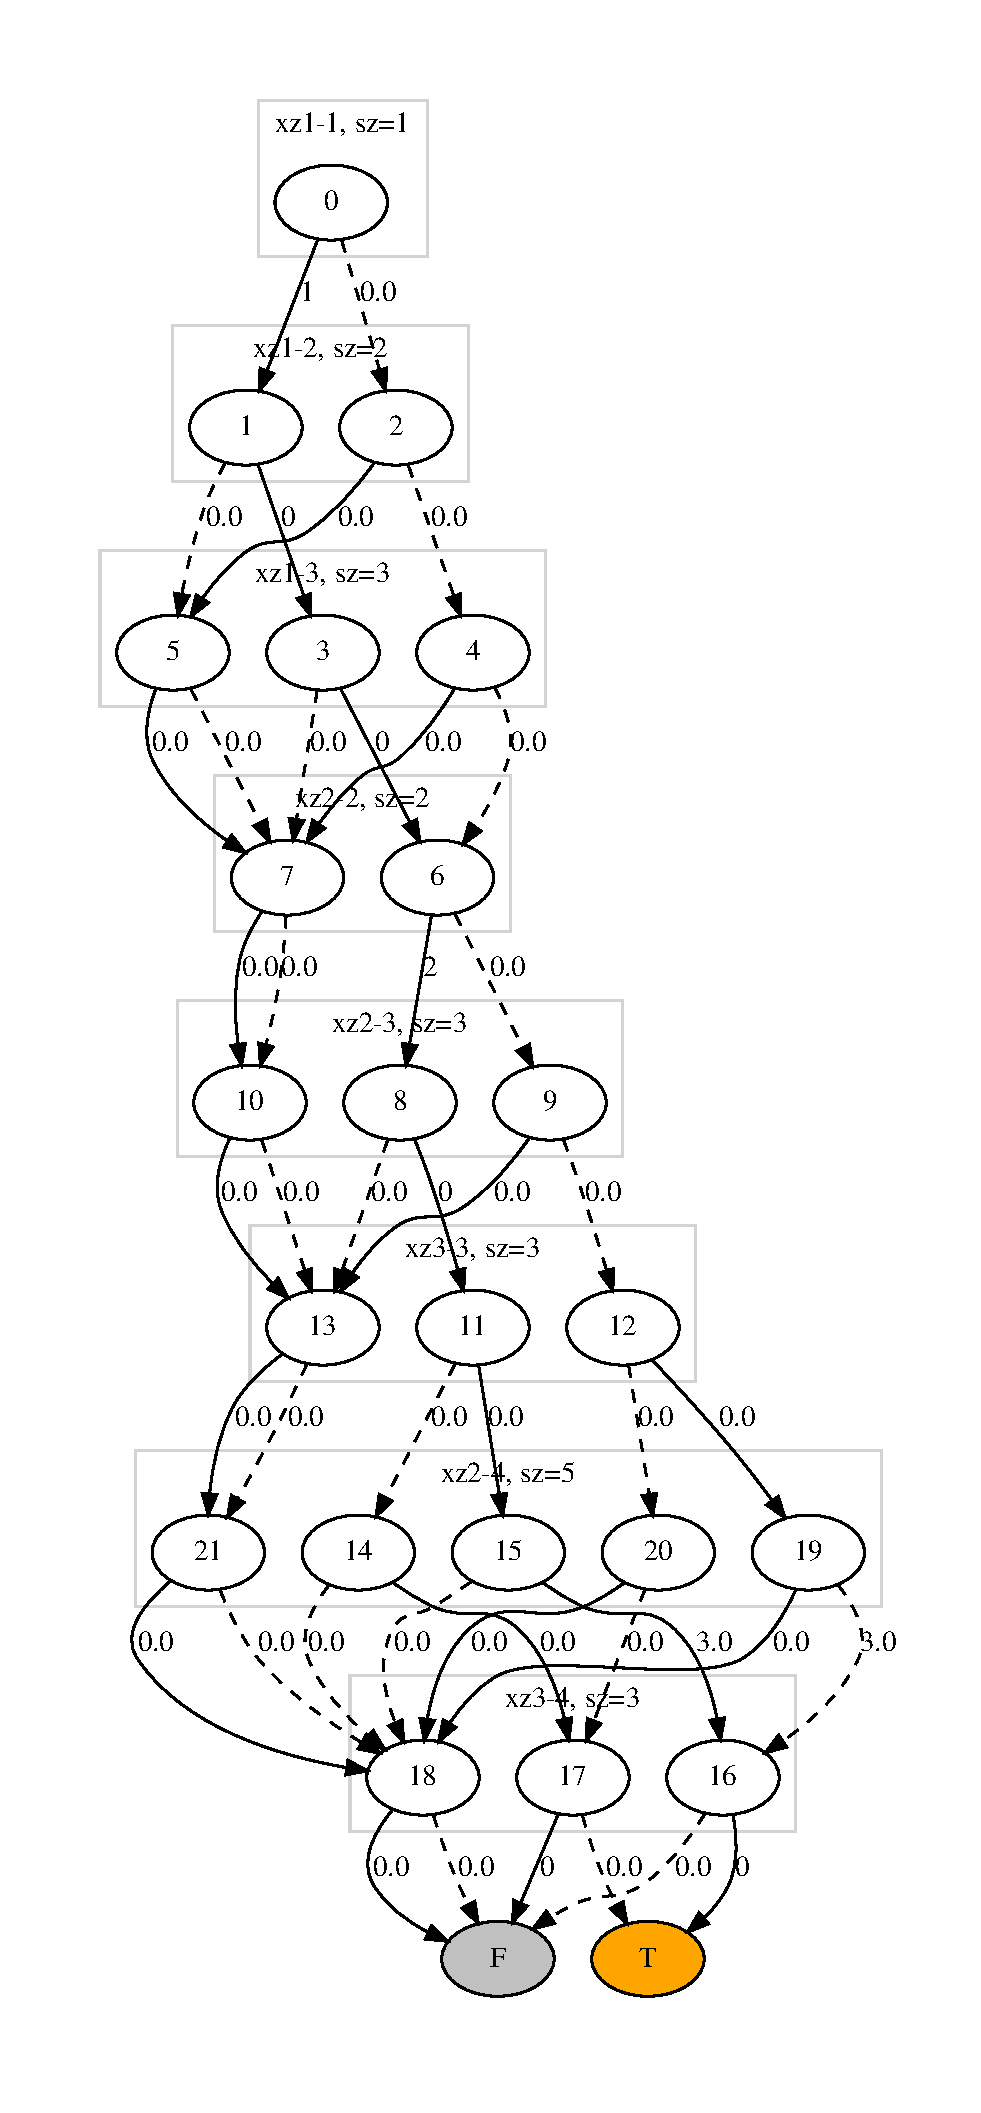
\includegraphics[height=\textheight]{./A_aligned.dot.pdf}
    \caption{Availability BDD}\label{fig:availA}
  \end{subfigure}
  \caption{BDDs generated to encode the instance from Figure \ref{fig:problem}: after alignment.}
\end{figure}

So, I can generate an intersection BDD (Figure \ref{fig:intDD}) and the corresponding MIP:\\

\begin{figure}[h!]
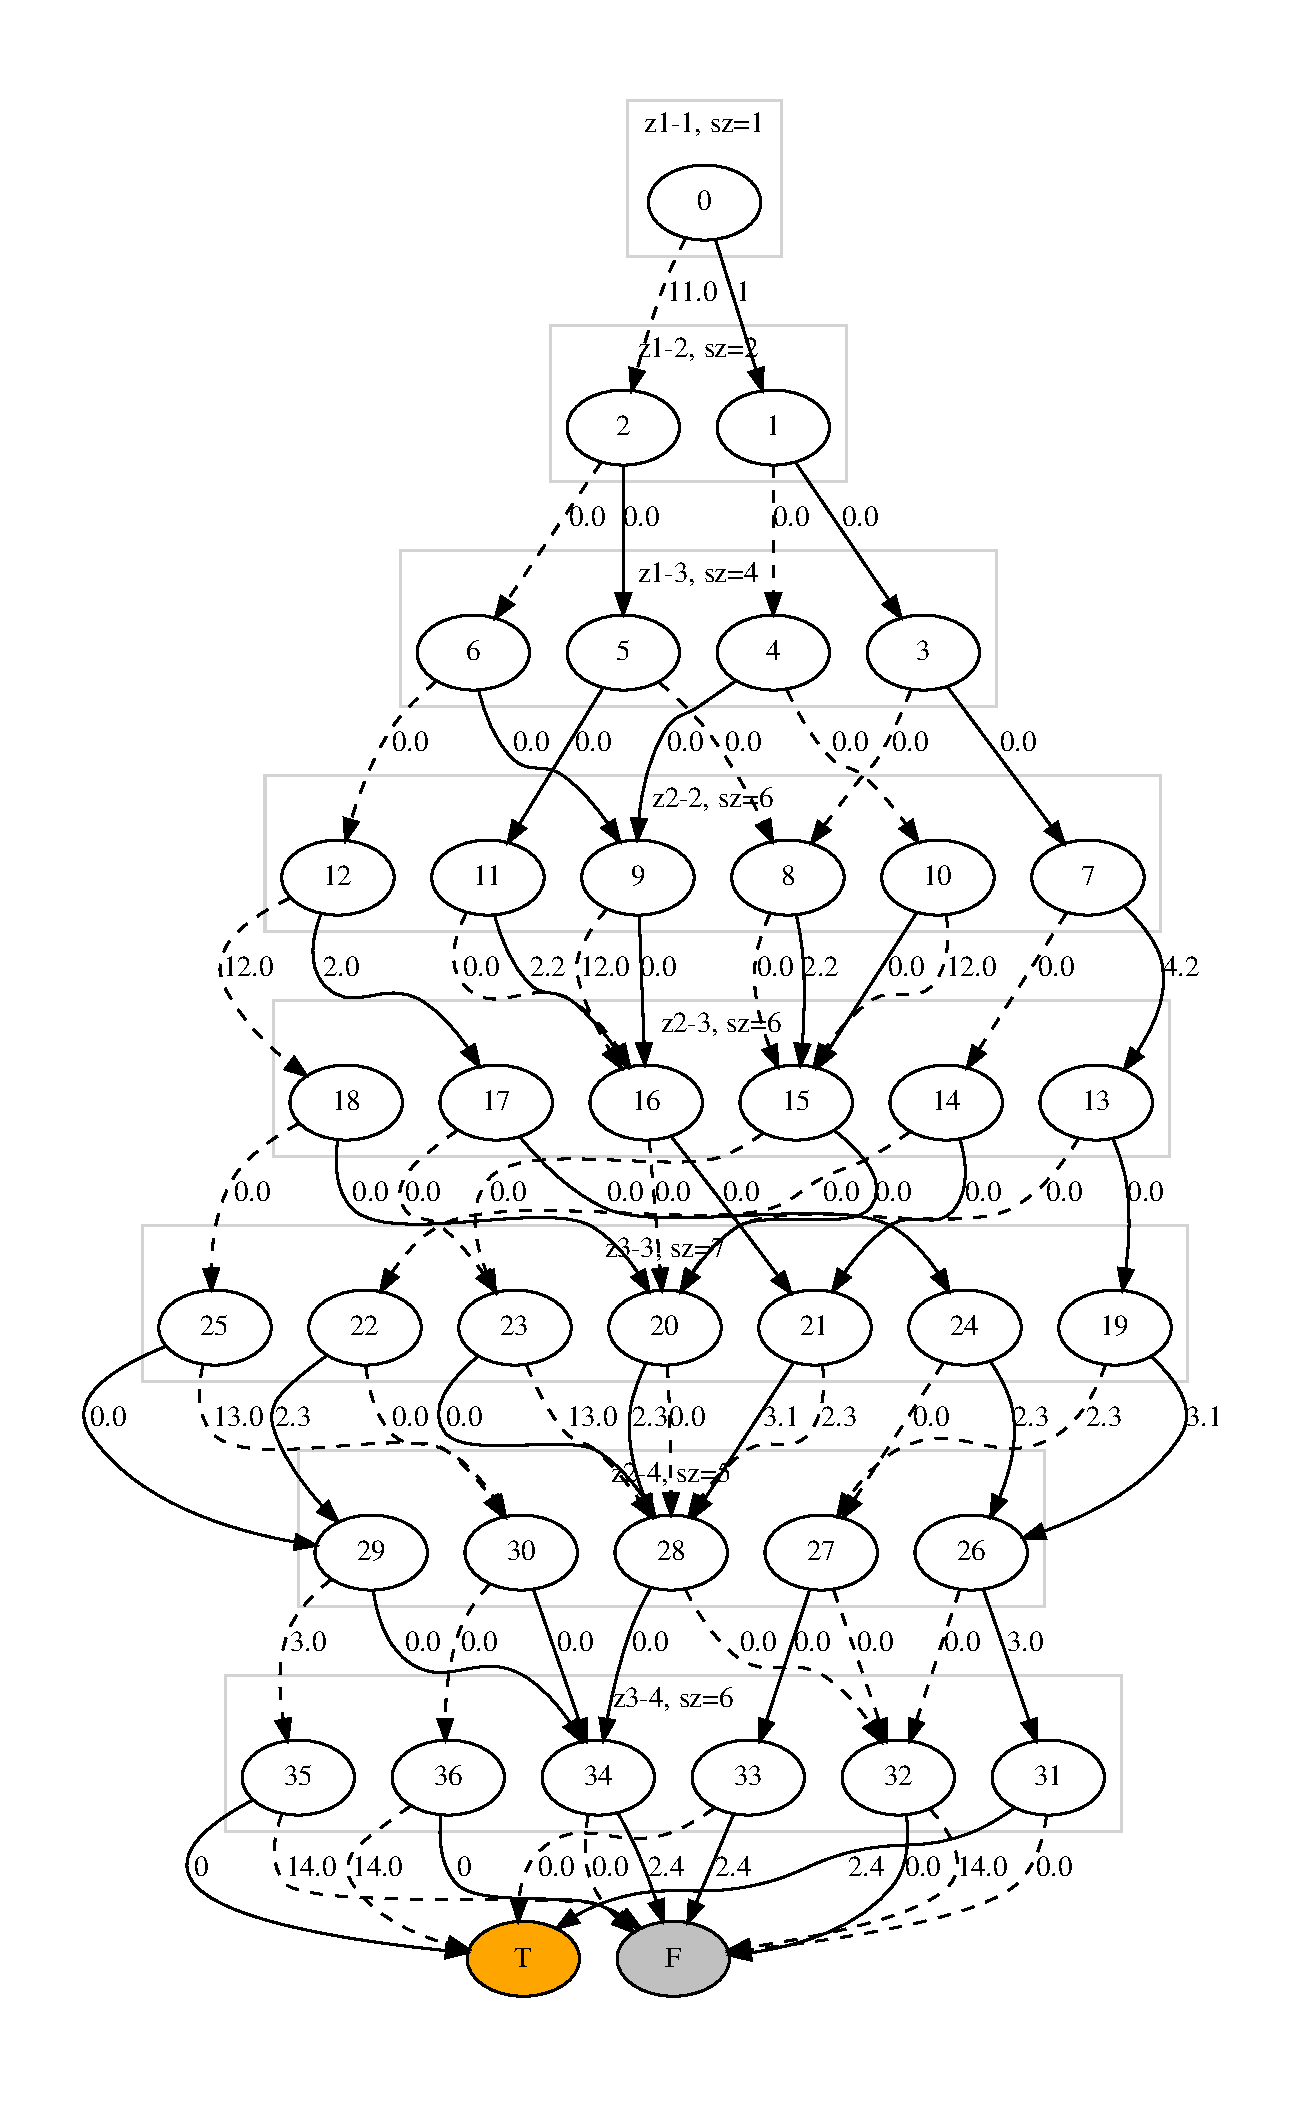
\includegraphics[width=0.9\textwidth]{./intersection.dot.pdf}
\caption{An intersection diagram for 'availability' and 'covering' DDs.}
\label{fig:intDD}
\end{figure}

The objective is:
\begin{flalign*}
\textrm{Minimize: } & v_{0 \rightarrow 1, h} + 11.0 v_{0 \rightarrow 2, l} + 12.0 v_{10 \rightarrow 15, l} + 2.0 v_{12 \rightarrow 17, h} + 12.0 v_{12 \rightarrow 18, l} + 12.0 v_{9 \rightarrow 16, l} + \\
& 2.2 v_{11 \rightarrow 16, h} + 4.2 v_{7 \rightarrow 13, h} + 2.2 v_{8 \rightarrow 15, h} + 13.0 v_{23 \rightarrow 28, l} + 3.1 v_{21 \rightarrow 28, h} + 2.3 v_{21 \rightarrow 28, l} + 2.3 v_{22 \rightarrow 29, h} +\\
& 2.3 v_{24 \rightarrow 26, h} + 2.3 v_{20 \rightarrow 28, h} + 13.0 v_{25 \rightarrow 30, l} + 3.1 v_{19 \rightarrow 26, h} + 2.3 v_{19 \rightarrow 27, l} + 3.0 v_{26 \rightarrow 31, h} + 3.0 v_{29 \rightarrow 35, l} +\\
& 14.0 v_{36 \rightarrow T, l} + 2.4 v_{34 \rightarrow F, h} + 14.0 v_{32 \rightarrow F, l} + 2.4 v_{33 \rightarrow F, h} + 2.4 v_{31 \rightarrow T, h} + 14.0 v_{35 \rightarrow F, l},
\end{flalign*}

under the constraints, presented in Table \ref{tab:NFconstr}. Obviously, here I
have continuous variables only.

\begin{table}[ht]
\caption{Network flow constraints (for the intersection BDD).}
 \begin{tabular}{l l}
 \textbf{Type} & \textbf{Constraint}\\\hline\\
   cont-at-0 & $-1.0 v_{0 \rightarrow 1, h} -1.0 v_{0 \rightarrow 2, l} = -1.0$\\
   cont-at-2 & $v_{0 \rightarrow 2, l} -1.0 v_{2 \rightarrow 5, h} -1.0 v_{2 \rightarrow 6, l} = 0.0$\\
   cont-at-1 & $v_{0 \rightarrow 1, h} -1.0 v_{1 \rightarrow 3, h} -1.0 v_{1 \rightarrow 4, l} = 0.0$\\
   cont-at-4 & $v_{1 \rightarrow 4, l} -1.0 v_{4 \rightarrow 9, h} -1.0 v_{4 \rightarrow 10, l} = 0.0$\\
   cont-at-5 & $v_{2 \rightarrow 5, h} -1.0 v_{5 \rightarrow 11, h} -1.0 v_{5 \rightarrow 8, l} = 0.0$\\
   cont-at-3 & $v_{1 \rightarrow 3, h} -1.0 v_{3 \rightarrow 7, h} -1.0 v_{3 \rightarrow 8, l} = 0.0$\\
   cont-at-6 & $v_{2 \rightarrow 6, l} -1.0 v_{6 \rightarrow 9, h} -1.0 v_{6 \rightarrow 12, l} = 0.0$\\
   cont-at-10 & $v_{4 \rightarrow 10, l} -1.0 v_{10 \rightarrow 15, h} -1.0 v_{10 \rightarrow 15, l} = 0.0$\\
   cont-at-12 & $v_{6 \rightarrow 12, l} -1.0 v_{12 \rightarrow 17, h} -1.0 v_{12 \rightarrow 18, l} = 0.0$\\
   cont-at-9 & $v_{4 \rightarrow 9, h} + v_{6 \rightarrow 9, h} -1.0 v_{9 \rightarrow 16, h} -1.0 v_{9 \rightarrow 16, l} = 0.0$\\
   cont-at-11 & $v_{5 \rightarrow 11, h} -1.0 v_{11 \rightarrow 16, h} -1.0 v_{11 \rightarrow 16, l} = 0.0$\\
   cont-at-7 & $v_{3 \rightarrow 7, h} -1.0 v_{7 \rightarrow 13, h} -1.0 v_{7 \rightarrow 14, l} = 0.0$\\
   cont-at-8 & $v_{5 \rightarrow 8, l} + v_{3 \rightarrow 8, l} -1.0 v_{8 \rightarrow 15, h} -1.0 v_{8 \rightarrow 15, l} = 0.0$\\
   cont-at-18 & $v_{12 \rightarrow 18, l} -1.0 v_{18 \rightarrow 20, h} -1.0 v_{18 \rightarrow 25, l} = 0.0$\\
   cont-at-13 & $v_{7 \rightarrow 13, h} -1.0 v_{13 \rightarrow 19, h} -1.0 v_{13 \rightarrow 20, l} = 0.0$\\
   cont-at-17 & $v_{12 \rightarrow 17, h} -1.0 v_{17 \rightarrow 24, h} -1.0 v_{17 \rightarrow 23, l} = 0.0$\\
   cont-at-16 & $v_{9 \rightarrow 16, h} + v_{9 \rightarrow 16, l} + v_{11 \rightarrow 16, h} + v_{11 \rightarrow 16, l} -1.0 v_{16 \rightarrow 21, h} -1.0 v_{16 \rightarrow 20, l} = 0.0$\\
   cont-at-14 & $v_{7 \rightarrow 14, l} -1.0 v_{14 \rightarrow 21, h} -1.0 v_{14 \rightarrow 22, l} = 0.0$\\
   cont-at-15 & $v_{10 \rightarrow 15, h} + v_{10 \rightarrow 15, l} + v_{8 \rightarrow 15, h} + v_{8 \rightarrow 15, l} -1.0 v_{15 \rightarrow 20, h} -1.0 v_{15 \rightarrow 23, l} = 0.0$\\
   cont-at-23 & $v_{17 \rightarrow 23, l} + v_{15 \rightarrow 23, l} -1.0 v_{23 \rightarrow 28, h} -1.0 v_{23 \rightarrow 28, l} = 0.0$\\
   cont-at-21 & $v_{16 \rightarrow 21, h} + v_{14 \rightarrow 21, h} -1.0 v_{21 \rightarrow 28, h} -1.0 v_{21 \rightarrow 28, l} = 0.0$\\
   cont-at-22 & $v_{14 \rightarrow 22, l} -1.0 v_{22 \rightarrow 29, h} -1.0 v_{22 \rightarrow 30, l} = 0.0$\\
   cont-at-24 & $v_{17 \rightarrow 24, h} -1.0 v_{24 \rightarrow 26, h} -1.0 v_{24 \rightarrow 27, l} = 0.0$\\
   cont-at-20 & $v_{18 \rightarrow 20, h} + v_{13 \rightarrow 20, l} + v_{16 \rightarrow 20, l} + v_{15 \rightarrow 20, h} -1.0 v_{20 \rightarrow 28, h} -1.0 v_{20 \rightarrow 28, l} = 0.0$\\
   cont-at-25 & $v_{18 \rightarrow 25, l} -1.0 v_{25 \rightarrow 29, h} -1.0 v_{25 \rightarrow 30, l} = 0.0$\\
   cont-at-19 & $v_{13 \rightarrow 19, h} -1.0 v_{19 \rightarrow 26, h} -1.0 v_{19 \rightarrow 27, l} = 0.0$\\
   cont-at-30 & $v_{22 \rightarrow 30, l} + v_{25 \rightarrow 30, l} -1.0 v_{30 \rightarrow 34, h} -1.0 v_{30 \rightarrow 36, l} = 0.0$\\
   cont-at-26 & $v_{24 \rightarrow 26, h} + v_{19 \rightarrow 26, h} -1.0 v_{26 \rightarrow 31, h} -1.0 v_{26 \rightarrow 32, l} = 0.0$\\
   cont-at-27 & $v_{24 \rightarrow 27, l} + v_{19 \rightarrow 27, l} -1.0 v_{27 \rightarrow 33, h} -1.0 v_{27 \rightarrow 32, l} = 0.0$\\
   cont-at-28 & $v_{23 \rightarrow 28, h} + v_{23 \rightarrow 28, l} + v_{21 \rightarrow 28, h} + v_{21 \rightarrow 28, l} + v_{20 \rightarrow 28, h} + v_{20 \rightarrow 28, l} -1.0 v_{28 \rightarrow 34, h} -1.0 v_{28 \rightarrow 32, l} = 0.0$\\
   cont-at-29 & $v_{22 \rightarrow 29, h} + v_{25 \rightarrow 29, h} -1.0 v_{29 \rightarrow 34, h} -1.0 v_{29 \rightarrow 35, l} = 0.0$\\
   cont-at-36 & $v_{30 \rightarrow 36, l} -1.0 v_{36 \rightarrow F, h} -1.0 v_{36 \rightarrow T, l} = 0.0$\\
   cont-at-34 & $v_{30 \rightarrow 34, h} + v_{28 \rightarrow 34, h} + v_{29 \rightarrow 34, h} -1.0 v_{34 \rightarrow F, h} -1.0 v_{34 \rightarrow F, l} = 0.0$\\
   cont-at-32 & $v_{26 \rightarrow 32, l} + v_{27 \rightarrow 32, l} + v_{28 \rightarrow 32, l} -1.0 v_{32 \rightarrow F, h} -1.0 v_{32 \rightarrow F, l} = 0.0$\\
   cont-at-33 & $v_{27 \rightarrow 33, h} -1.0 v_{33 \rightarrow F, h} -1.0 v_{33 \rightarrow T, l} = 0.0$\\
   cont-at-31 & $v_{26 \rightarrow 31, h} -1.0 v_{31 \rightarrow T, h} -1.0 v_{31 \rightarrow F, l} = 0.0$\\
   cont-at-35 & $v_{29 \rightarrow 35, l} -1.0 v_{35 \rightarrow T, h} -1.0 v_{35 \rightarrow F, l} = 0.0$\\
   cont-at-T & $v_{36 \rightarrow T, l} + v_{33 \rightarrow T, l} + v_{31 \rightarrow T, h} + v_{35 \rightarrow T, h} = 1.0$\\
   cont-at-F & $v_{36 \rightarrow F, h} + v_{34 \rightarrow F, h} + v_{34 \rightarrow F, l} + v_{32 \rightarrow F, h} + v_{32 \rightarrow F, l} + v_{33 \rightarrow F, h} + v_{31 \rightarrow F, l} + v_{35 \rightarrow F, l} = 0.0$
 \end{tabular}
 \label{tab:NFconstr}
\end{table}

\subsection{A quick cross-check}
\label{sec:org3dc7b5f}
Of course, I'd like to cross-check somehow. E.g., I can just solve each of
the three models and make sure the optimal objective coincide. Indeed:
\begin{verbatim}
Opt statuses are: 2, 2, 2
('optimal' is encoded by 2)
Optimal objectives are:
Simple MIP: 6.3
CPP MIP:    6.3
NF (linear):6.3
\end{verbatim}


Here are, e.g., nonzero variables for the CPP MIP (\texttt{-1} encodes \textbf{True}
terminal node).

\begin{verbatim}
link_z1-1: 1.0
A_vh0_1: 1.0
link_z1-2: 1.0
A_vh1_3: 1.0
link_z1-3: 1.0
A_vh3_6: 1.0
A_vl6_9: 1.0
A_vl9_12: 1.0
A_vl12_14: 1.0
link_z3-3: 1.0
A_vh14_16: 1.0
link_z3-4: 1.0
A_vh16_-1: 1.0
C_vh0_1: 1.0
C_vh1_3: 1.0
C_vl3_4: 1.0
C_vh4_6: 1.0
C_vl6_8: 1.0
C_vh8_10: 1.0
C_vl10_11: 1.0
C_vh11_-1: 1.0
\end{verbatim}

This implies locating facilities \textcircled{1} and \textcircled{3}, and must
carry the cost \(1+3\) for location plus the overlap of \(2.3\) for overlapping at
customer 3. Seems to work: \(1+3+2.3=6.3\) (I am looking at Figure \ref{fig:problem}).

\section{The problem: intersection DD seems to blow up.}
\label{sec:org68588f8}
What I have done is a very simple experiment: I generated 15 random instances
for each of several problem sizes -- say, with number of facilities being
\(n=3,4,5,6\), and number of customers \(m=2n\) (in every case). Then, diagram sizes
(\(A\) for availability and \(C\) for covering), along with the number of variables
in the plain MIP grow reasonably fast (Figure \ref{fig:ACsizes}). However,
intersection BDD just blows up (Figure \ref{fig:intSizes} -- note I had to draw
it in \textbf{logarithmic} scale), and so does the runtime of what I am doing (Figure
\ref{fig:runtimes}). Practically, for the way I am generating instances, it
seems I can't get to the point where making a BDD would be beneficial as
compared to a plain MIP (it has to have a huge number of variables, right?) --
solution just seem to take too long even for moderate problem sizes (I mean, \(n\)
and \(m\))\ldots{} That is, maybe even our simplified-problem based approach
outperforms, say, some baseline 'sifting' method, but it seems the very idea of
constructing a BDD is quite tough to implement, at least in such straightforward
way. What I was thinking:
\begin{itemize}
\item maybe there is a (performance) bug somewhere, there is always such a
possibility. Also, maybe rewriting the whole story in C++ or Julia would help.
It is not difficult conceptually, but will take time -- and, most importantly,
Figure \ref{fig:intSizes} suggests it won't help fundamentally. So, to me,
this seems \emph{not} the best starting point.
\item in particular, maybe something breaks down when I start to work with
\emph{weighted} DDs and that many variables. (we were experimenting with up to 25
variables, now I can have, like, hundreds -- and think it is a moderate-sized
instance\ldots{}) So, I might want to look into a more careful testing and
optimization of operations with weighted DDs. I kind of checked that
weighted-swap/sift work (in a sense of the same terminal nodes and paths), but
maybe the resulting DDs are still too big?
\item we might want to think about the problem structure. What case would make it
especially difficult for a plain MIP formulation? (I remember discussing many
overlaps + non-convex structure of \(g\)).
\item Like I mentioned, I'd appreciate any comments, but I will keep thinking what we can do.
\end{itemize}

\begin{figure}
  \begin{subfigure}{0.45\textwidth}
    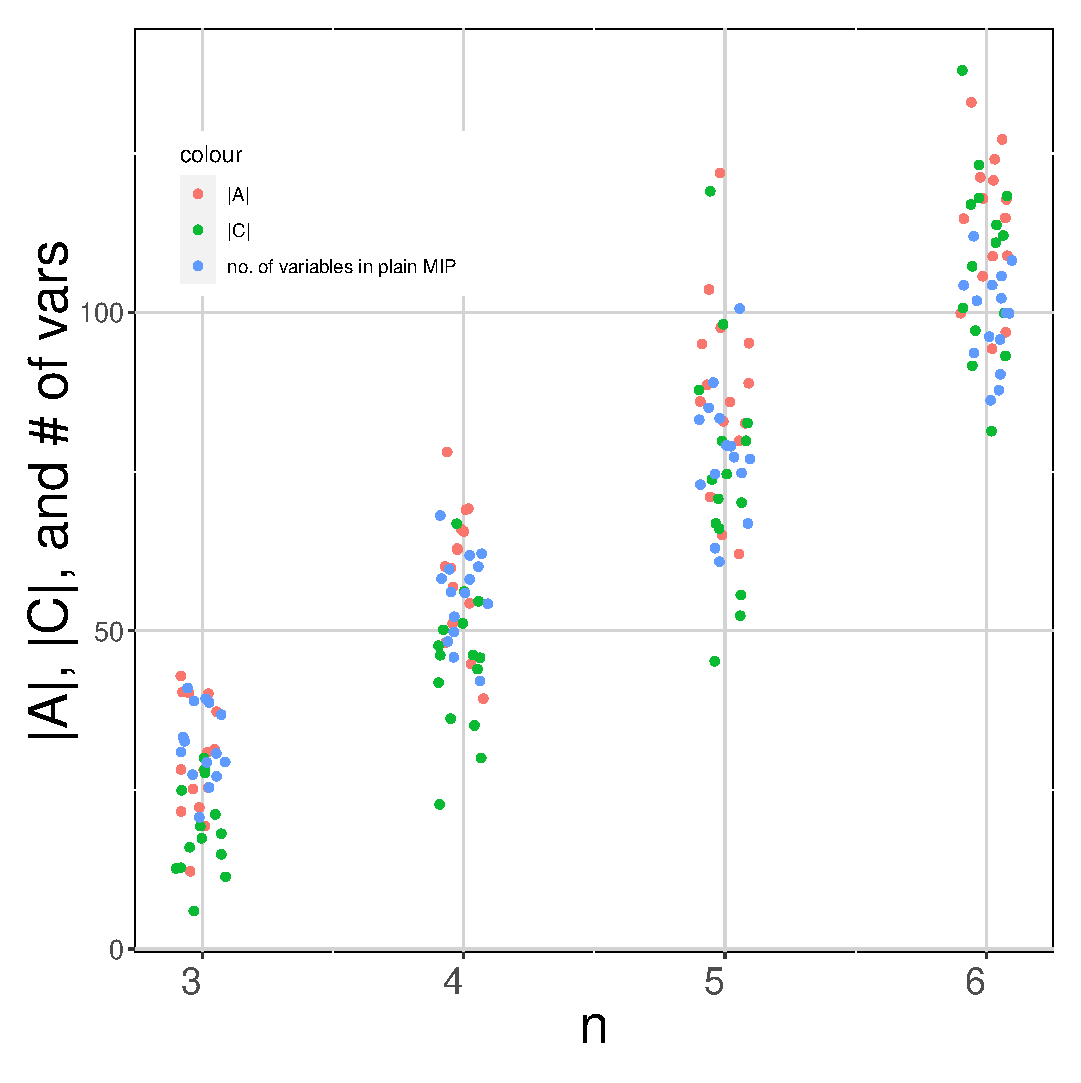
\includegraphics[width=\textwidth]{AandCsizes.eps}
    \caption{Diagram growth as number of facilities increases.}
    \label{fig:ACsizes}
  \end{subfigure}
  \hfill
  \begin{subfigure}{0.45\textwidth}
    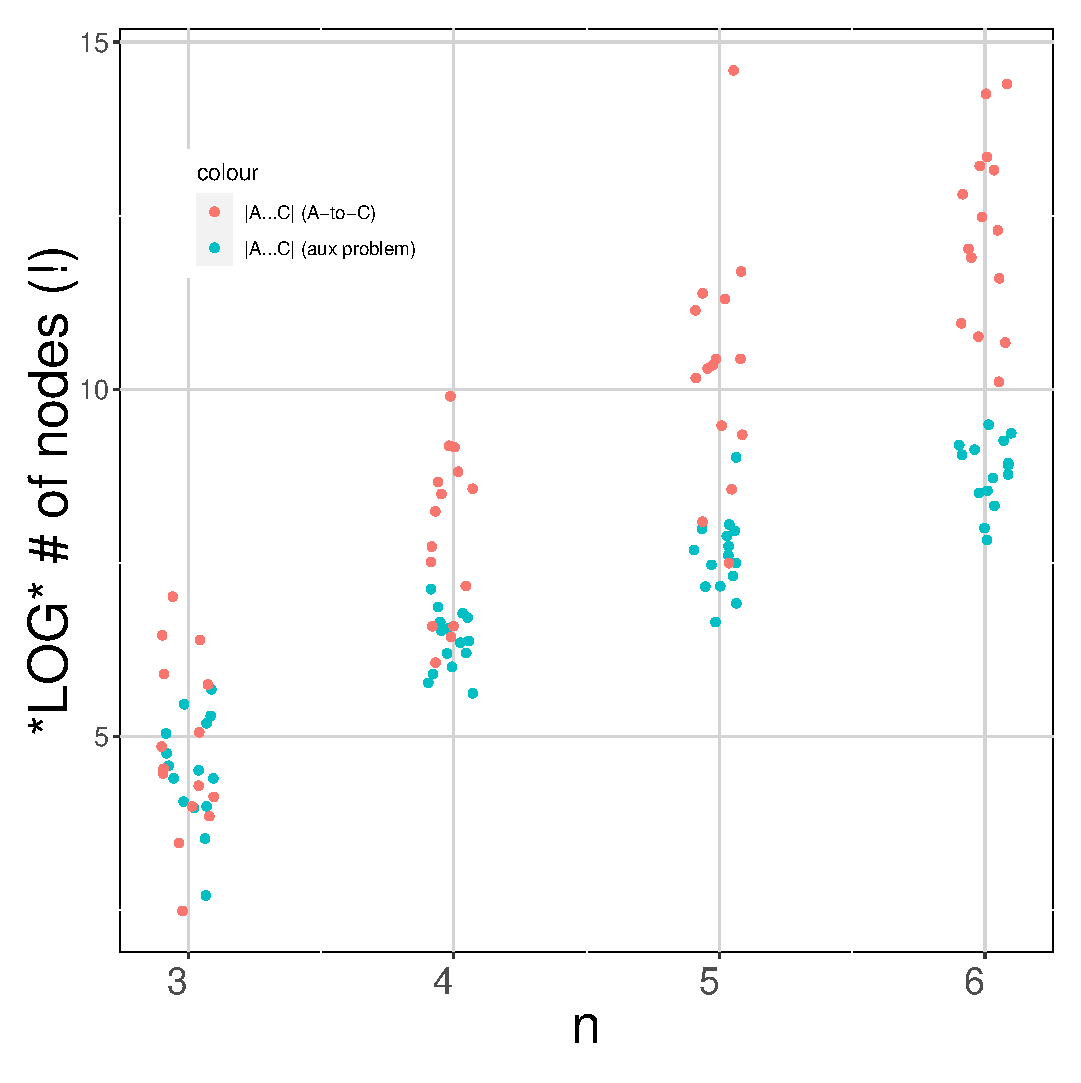
\includegraphics[width=\textwidth]{inter_size.eps}
    \caption{Intersection diagram growth as number of facilities increases.}
    \label{fig:intSizes}
  \end{subfigure}
\end{figure}

\begin{figure}
\center
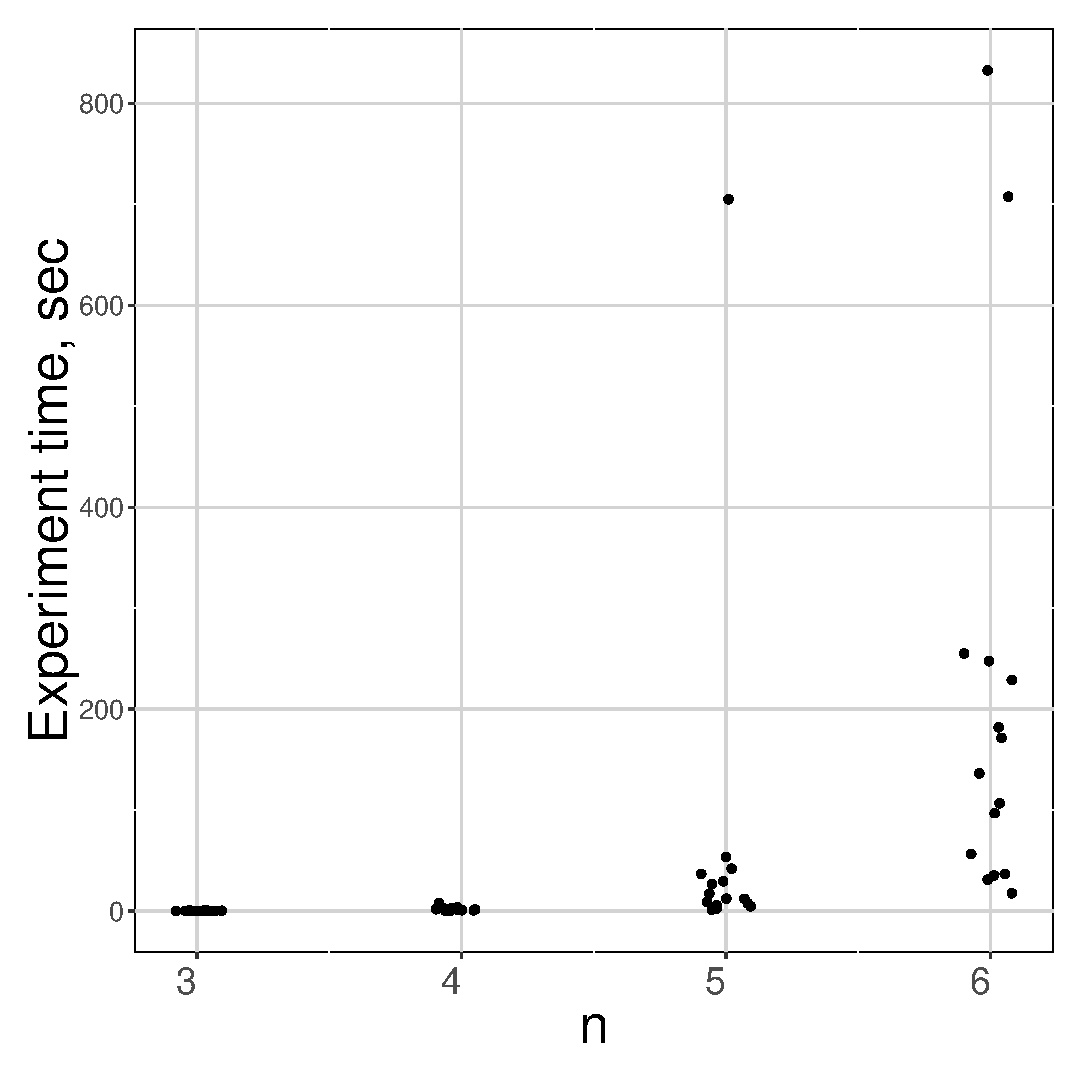
\includegraphics[width=0.7\textwidth]{runtimes.eps}
\caption{Experiment runtimes, seconds}
\label{fig:runtimes}
\end{figure}
\end{document}